\chapter{Methodology}\label{ch:3}
This chapter delineates the comprehensive and systematic methodology employed to develop and evaluate a sophisticated classification pipeline capable of determining course equivalency from domain-specific textual data. The methodological framework presented here is the result of an evolutionary research process that progressed through two distinct phases.

The investigation commenced with an initial, exploratory phase to assess the feasibility of using Large Language Models (LLMs) as end-to-end classifiers, as introduced in Section~\ref{ch:2.4}. This direct approach was conceived as a benchmark, leveraging a small, manually curated dataset. The findings from this stage were critical; they demonstrated the potential of modern LLMs but also confirmed the significant limitations previously discussed~\cite{pardos-articulation-2019}.

These challenges fundamentally shaped the subsequent research, motivating the development of the more robust and scalable framework that is the primary focus of this thesis. The foundational principle of this final pipeline is to utilize state-of-the-art deep embedding models not as end-to-end classifiers, but as highly sophisticated feature extraction engines. In this paradigm, each course description is converted into a high-dimensional numerical vector that encapsulates its rich semantic content~\cite{devlin2019bertpretrainingdeepbidirectional}. By pre-processing and storing these embeddings, the framework eliminates the need to repeatedly process raw text through costly APIs or resource hungry compute nodes, drastically reducing computational overhead and making the system inherently more scalable for real-world applications. The narrative of this chapter follows this logical evolution, detailing the data acquisition, model architectures, training protocols, and evaluation frameworks for each stage of the research.

\section{Initial Approach: Direct LLM Classification}\label{ch:3.1}
As outlined in Section~\ref{ch:2.4}, the research began with an exploratory phase to establish a performance baseline using a direct, end-to-end LLM classification approach. This was a pragmatic first step, as the larger Program Pathways Mapper (PPM) dataset was not yet available, making a focused, smaller-scale investigation the most logical starting point. This initial methodology treated the LLM as a holistic reasoning engine, and its findings were critical in shaping the decoupled pipeline that followed.

\subsection{Initial Data Corpus and Pre-processing}\label{ch:3.1.1}
The dataset for this initial evaluation was constructed to represent a challenging, real-world scenario using publicly available data from ASSIST, as described in Chapter~\ref{ch:2}. The process began by identifying five required lower-division courses for the Computer Science major at San Francisco State University (SFSU). Articulation agreements were found for these courses across 63 different California public colleges and universities. The raw course data, consisting of department codes, numbers, titles, descriptions, and all metadata, was manually collected from each college's online catalog. This approach was chosen to allow for a comparison between using complete raw text versus more structured information for classification.

The initial dataset consisted of 228 equivalent course pairs based on articulation agreements. To create a more robust dataset for binary classification, this set was expanded by assuming symmetry and transitivity for course equivalency, which generated 5,660 equivalent pairs. An equivalent number of non-equivalent pairs was then generated by randomly pairing courses from different subjects. From this corpus, a final stratified random sample of 400 pairs (200 equivalent and 200 non-equivalent) was created to serve as the evaluation set.

\subsection{Model Selection and Prompt Engineering}\label{ch:3.1.2}
After an initial review of various LLMs for their ability to reliably generate structured data, Google's PaLM2 and its successor, Gemini Pro v1.0, were selected for this phase. This decision was based on their accessibility via a free-tier API and their consistent ability to produce well-formatted, structured data from unprocessed text.

A systematic, iterative prompt engineering process (Figure~\ref{fig:prompt_engineering_process}) was used to develop effective prompts for both data extraction and final classification. This involved refining simple prompts based on established design principles~\cite{ye2024promptengineeringpromptengineer,ppp,peg}. The final prompts were highly structured, containing a preamble, raw data, formatting instructions, a JSON schema, and a postamble. Despite this careful refinement, the structured data extraction, particularly for deducing course topics, remained a challenge and was prone to occasional errors.

\begin{figure}[tb]
    \captionsetup{skip=5pt}
    \centering
    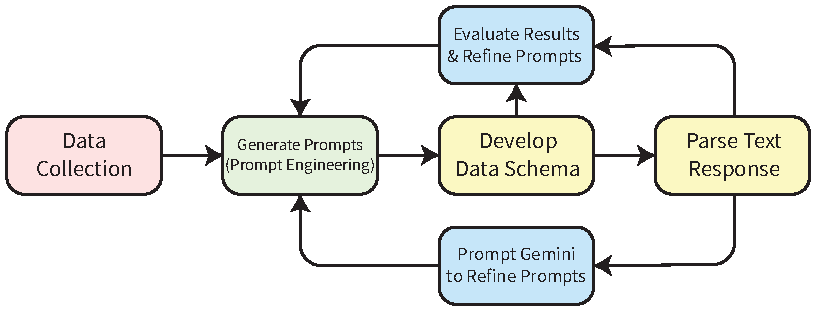
\includegraphics[scale=1,trim={0 0 0 0},clip]{pef.pdf}
    \caption{Prompt Engineering Process}
    \label{fig:prompt_engineering_process}
\end{figure}

\subsection{Classification and Evaluation Findings}
The core of this phase involved pairwise course assessments using Gemini Pro. The evaluation was structured to explore different scenarios:
\begin{itemize}
    \item \textbf{Input Data}: Evaluations were conducted using both the full, raw course text and a structured format with only the course discipline and LLM-extracted topics.
    \item \textbf{Classification Tasks}: Three distinct classification tasks were designed: a standard binary classification, a three-class model adding an ``unsure'' category, and a four-class model also including ``insufficient data''.
\end{itemize}

The model achieved a notable 90.5\% accuracy on the binary classification task using the full raw text, confirming that unprocessed text was a superior input format. Performance degraded when using only the structured topics, likely due to errors from the LLM's extraction process. The multi-class experiments proved valuable for simulating the ambiguity a human advisor might face, demonstrating a method for isolating cases requiring manual review.

Crucially, and as summarized in Section~\ref{ch:2.4}, this investigation confirmed several fundamental weaknesses in the direct LLM approach, making it unsuitable for a scalable production system~\cite{pardos-articulation-2019, shiferaw2024}. The method provided no confidence scores or granular similarity metrics, preventing the ranking of course pairs or identifying ``close but not equivalent'' courses~\cite{reimers-2019-sentence-bert}. The approach was also computationally expensive and the prompts were highly model-specific, necessitating significant rework if the underlying model were changed. These limitations directly motivated a pivot in methodology towards the decoupled, embedding-based pipeline detailed in the following sections.

\section{The PPM Corpus and Data Preparation}\label{ch:3.2}
The limitations identified in the initial study necessitated a larger, more comprehensive dataset to robustly train and evaluate the new methodology. This data corpus was procured in partnership with the Program Pathways Mapper (PPM), which was a critical step that enabled the full-scale implementation of the decoupled pipeline. This section characterizes the PPM corpus and details its preparation.

\subsection{Dataset Characterization and Partitioning}\label{ch:3.2.1}
The PPM corpus initially contained 2,217 courses, each labeled with a Course Identification Numbering System (C-ID) code serving as ground truth. A critical filtering step was first applied, removing all C-ID classes with fewer than four associated courses. This was essential to guarantee that both training and test sets would contain at least one equivalent pair for every class, a necessary condition for the fine-tuning process. This resulted in a final corpus of 2,157 courses across 157 distinct C-ID classes.

This final dataset was partitioned into non-overlapping training and test sets using a stratified 50/50 split, with the C-ID code as the stratification key. This resulted in a training set of 1078 courses and a test set of 1079 courses, ensuring each of the 157 classes was represented in both subsets. The test set was held in reserve for the final, unbiased evaluation of the complete pipeline. The training set served a dual purpose: generating (anchor, positive, negative) triplets for fine-tuning and generating binary pairs for validation during the fine-tuning process. This allows for robust validation on the primary task (binary classification) without data leakage from the optimization task (triplet distance minimization).

\subsection{Input Document Normalization}\label{ch:3.2.2}
This research deliberately eschewed standard text pre-processing like lowercasing or stop-word removal to simulate real-world use where input data may be imperfect. The methodology relies on the robustness of modern transformer models to handle this ``raw'' text~\cite{devlin2019bertpretrainingdeepbidirectional}. Instead of cleaning, a normalization step created a consistent input document for each course. A new field, ``Formatted Course Info,'' was generated by concatenating four key pieces of information: department name, course number, title, and full description.  An example of the resulting ``Formatted Course Info'' string is shown in Listing~\ref{lst:formatted_info}.  This concatenated string serves as the single document representation for each course and is the direct input for the embedding process, ensuring all relevant context is preserved.
\begin{lstlisting}[
    language=bash,
    caption={Example of a "Formatted Course Info" String},
    label={lst:formatted_info},
    basicstyle=\ttfamily\small,
    breaklines=true,
    breakatwhitespace=true,
    postbreak=\mbox{\textcolor{red}{$\hookrightarrow$}\space},
    captionpos=b,
    frame=single,
    xleftmargin=2em,
    framexleftmargin=1.5em
]
CSC-101 Introduction to Computing (Units: 3)
A comprehensive introduction to computing and programming. No prior programming experience is required. Explore the use of computing in everyday life and its impact on our society, and apply foundational ideas of computing to frame a problem and devise a solution using Java programming language.
\end{lstlisting}

\subsection{Data Structuring for Fine-Tuning}\label{ch:3.2.3}
The triplet loss functions used in this research operate on (anchor, positive, negative) triplets and are designed to form these triplets on-the-fly from within each mini-batch of (text, label) pairs~\cite{reimers-2019-sentence-bert,sbertLossOverview}. A crucial constraint of these loss functions is that the training data must contain at least two examples for each class label to form a valid (anchor, positive) pair~\cite{sbertLosses}. A simple random sampling approach could easily create mini-batches that fail this constraint, leading to an inefficient training process.

To mitigate this, this research leveraged a specialized feature of the sentence-transformers library: the \verb|GroupByLabelBatchSampler|. This sampler, activated during trainer configuration, ensures that each mini-batch is constructed by grouping samples with the same label~\cite{sbertSamplers}. This guarantees every batch contains the necessary class diversity to form valid and informative triplets, demonstrating that the data loading stage is intrinsically linked to the fine-tuning objective.

\section{Embedding Model Selection and Fine-Tuning}\label{ch:3.3}
A central hypothesis of this research is that a generic, pre-trained deep embedding model can be fine-tuned to produce highly specialized embeddings for the domain of course descriptions, providing a more discriminative feature representation than off-the-shelf models. This section details the architecture, learning objective, and training protocol used to achieve this adaptation via deep metric learning.

\subsection{Model Selection}\label{ch:3.3.1}
The research began with a broad analysis of open-source embedding models, previously summarized in Table~\ref{tbl:taxonomy}, to identify candidates for in-depth study. The initial models reviewed spanned a range of parameter sizes and characteristics (Table~\ref{tbl:emb_models}).

\begin{table}[!tb]
    \captionsetup{skip=5pt}
    \centering
    \caption{Initial Embedding Model Review}
    \label{tbl:emb_models}
    \begin{tabular}{lcccc}
        \toprule
        Model Name                 & Rank$^{*}$ & Params$^{\dagger}$ & Dims & Acc             \\
        \midrule
        GIST-small-Embedding-v0    & 41         & 33                 & 384  & 0.9759          \\
        bge-small-en-v1.5          & 47         & 33                 & 384  & 0.9670          \\
        GIST-Embedding-v0          & 33         & 109                & 768  & 0.9768          \\
        bge-base-en-v1.5           & 35         & 109                & 768  & 0.9732          \\
        gte-base-en-v1.5           & 31         & 137                & 768  & 0.9732          \\
        mxbai-embed-large-v1       & 24         & 335                & 1024 & 0.9759          \\
        gte-large-en-v1.5          & 21         & 434                & 1024 & 0.9777          \\
        multilingual-e5-large-inst & 34         & 560                & 514  & 0.9670          \\
        stella\_en\_1.5B\_v5       & 3          & 1543               & 8192 & 0.9857          \\
        SFR-Embedding-2\_R         & 4          & 7111               & 4096 & \textbf{0.9839} \\
        Agte-Qwen2-7B-instruct     & 5          & 7613               & 3584 & 0.9804          \\
        nvidia/NV-Embed-v2         & 1          & 7851               & 4096 & 0.9831          \\
        \bottomrule
        \multicolumn{4}{p{6cm}}{\scriptsize $^{*}$ Huggingface Overall Leaderboard Rank} \\
        \multicolumn{4}{p{6cm}}{\scriptsize $^{\dagger}$ in Millions}
    \end{tabular}
\end{table}

To screen these models efficiently, a simple cosine similarity accuracy metric was used, which allowed for the rapid elimination of poorly performing models. While many models achieved high accuracy (sample mean of 0.9767), three were selected for primary analysis to represent a spectrum of sizes:
\begin{itemize}
    \item \verb|BAAI/bge-small-en-v1.5| (BGE): A high-performing small model.
    \item \verb|avsolatorio/GIST-Embedding-v0| (GIST): A medium-sized model.
    \item \verb|nvidia/NV-Embed-v2| (NVE): A large-scale model.
\end{itemize}
Later, \verb|Salesforce/SFR-Embedding-2_R| (SFR) was also included due to its strong performance on public leaderboards.

\subsection{Metric Learning with Batch Triplet Loss Functions}\label{ch:3.3.2}
To determine if performance could be improved, the BGE model was fine-tuned using a metric learning approach, which aims to learn an embedding space where geometric distance corresponds to semantic similarity~\cite{mohan2023deepmetriclearningcomputer}. This provides a more powerful and nuanced objective than simple classification, directly addressing a key limitation of the initial LLM approach.

\subsubsection{Theoretical Foundation of Triplet Loss}\label{ch:3.3.2.1}
First introduced by Yu, et al. for face recognition, Triplet Loss has been widely applied to supervised similarity learning~\cite{Yu2020}. It operates on (Anchor, Positive, Negative) triplets, with the goal of training the embedding function \(f(x)\) to map inputs into a vector space where the distance between an anchor (\(A\)) and a positive sample (\(P\)) is smaller than the distance to a negative sample (\(N\)) by at least a margin \(\alpha\)~\cite{Schroff_2015_CVPR, hermans2017defensetripletlossperson, mohan2023deepmetriclearningcomputer}. The mathematical formulation is given by:
\[ L(A,P,N)=\max(d(f(A),f(P))-d(f(A),f(N))+\alpha,0). \]
Here, \(d\) is the Euclidean distance. The \(\max()\) component ensures that loss is only incurred for triplets that violate the margin constraint. If a triplet already satisfies the margin, its loss is zero.

\subsubsection{Online Triplet Mining and Batch-based Losses}\label{ch:3.3.2.2}
A naive ``offline'' implementation of Triplet Loss that forms all possible triplets is computationally infeasible. A more effective approach is ``online'' mining, where informative triplets are selected on-the-fly from each mini-batch. These triplets can be categorized by difficulty:
\begin{itemize}
    \item \textbf{Easy Triplets}: Already satisfy the margin (\(d(A,P)+\alpha<d(A,N)\)). They result in zero loss and do not contribute to learning.
    \item \textbf{Semi-Hard Triplets}: The negative is further than the positive but within the margin (\(d(A,P)<d(A,N)<d(A,P)+\alpha\)). They have a positive loss and provide a stable gradient.
    \item \textbf{Hard Triplets}: The negative is closer than the positive (\(d(A,N)<d(A,P)\)). They produce the largest loss and strongest learning signal.
\end{itemize}

\subsubsection{Empirical Evaluation of Batch Triplet Loss Functions}\label{ch:3.3.2.3}
Recognizing that different mining strategies impact performance, this research empirically evaluated all four primary batch-based triplet loss implementations in the sentence-transformers library to identify the optimal strategy. The evaluated functions were:
\begin{itemize}
    \item \textbf{BatchAllTripletLoss}: Computes loss for all valid triplets in a batch. It is comprehensive but can be diluted by many ``easy'' triplets.
    \item \textbf{BatchSemiHardTripletLoss}: Considers only semi-hard triplets. This provides stable training but may converge slowly by ignoring the hardest examples.
    \item \textbf{BatchHardTripletLoss}: For each anchor, it uses the hardest positive and hardest negative. This can accelerate convergence but can also be ``temperamental'' and lead to a noisy optimization.
    \item \textbf{BatchHardSoftMarginTripletLoss}: A variation of BatchHardTripletLoss that does not require a specified margin, simplifying hyperparameter tuning.
\end{itemize}
The final model used for feature generation was trained with the loss function that demonstrated the best validation performance during this empirical evaluation.

\subsection{Optimization and Training Protocol}\label{ch:3.3.3}
The successful fine-tuning of a model with a challenging objective like \verb|BatchHardTripletLoss| depends on the optimizer and learning rate schedule. The components selected---AdamW and Cosine Annealing with Warm Restarts---were chosen as a cohesive framework for stable and effective learning.{\setlength{\emergencystretch}{5em}\par}

\subsubsection{Optimizer Selection: AdamW}\label{ch:3.3.3.1}
The optimization was performed using AdamW. AdamW is based on the Adam optimizer, which is effective and efficient, combining benefits from the momentum method and RMSprop~\cite{loshchilov2019decoupledweightdecayregularization}. Its per-parameter adaptive learning rate is well-suited for the noisy gradients from \verb|BatchHardTripletLoss|. AdamW improves upon standard Adam by decoupling the weight decay (L2 regularization) from the gradient update~\cite{loshchilov2019decoupledweightdecayregularization}. This fixes a flaw where the regularization effect was inconsistently applied, leading to better generalization and training stability, making it a superior choice for this complex training process~\cite{loshchilov2019decoupledweightdecayregularization}.

\subsubsection{Learning Rate Schedule: Cosine Annealing with Warm Restarts}\label{ch:3.3.3.2}
A dynamic learning rate schedule can significantly improve performance, even with an adaptive optimizer like AdamW~\cite{loshchilov2019decoupledweightdecayregularization}. This research employed the \verb|CosineAnnealingWarmRestarts| schedule. This schedule smoothly decays the learning rate following a cosine curve and incorporates "warm restarts," where the rate is periodically reset to its initial maximum~\cite{pytorchcosanneal, loshchilovhutter}. The learning rate \(\nu_t\) at epoch \(T_{\textrm{cur}}\) within a cycle of length \(T_i\) is:{\setlength{\emergencystretch}{5em}\par}
\[ \nu_t = \nu_{\textrm{min}} + \frac{1}{2}\left( \nu_{\textrm{max}} -\nu_{\textrm{min}} \right)\left(1 + \cos\left(\frac{T_{\textrm{cur}}}{T_{\textrm{max}}}\pi\right)\right) \]
This combination is a powerful strategy. The aggressive \verb|BatchHardTripletLoss| creates a complex loss surface with sharp, suboptimal local minima. When the model appears to converge, the warm restart ``kicks'' the optimizer out of the local minimum, allowing it to explore other regions of the loss landscape, while the subsequent smooth decay allows it to settle into a new, potentially better minimum. This synergistic framework of loss function, optimizer, and learning rate schedule is critical for training a highly discriminative model under these demanding conditions.

\section{Generating Course Embeddings}\label{ch:3.4}
Upon completion of model selection and fine-tuning, the selected models were used to transform the text corpus into structured numerical vectors. Operating in inference mode, each model processed the ``Formatted Course Info'' for every course in the training and test sets to generate a fixed-length embedding vector. This was performed for the models summarized in Table~\ref{tbl:emb}.

\begin{table}[!bt]
    \captionsetup{skip=5pt}
    \caption{Embedding Models \& PCA Explained Variance}
    \centering
    \resizebox{\columnwidth}{!}{
        \begin{tabular}{lcp{9em}p{5em}p{2.2em}p{2.2em}p{2.2em}}
            \toprule
            &           &                             &                          & \multicolumn{3}{c}{Explained Variance} \\
            &           & \centering\# of Parameters & \centering Embedding     & \multicolumn{3}{c}{(\# of PCs)} \\
            \cmidrule{5-7} Model Name     & Type Used\(^{*}\) & \centering (in Millions)   & \centering Dimensions & 70\%  & 80\% & 90\% \\
            \midrule
            BAAI/bge-small-en-v1.5        & OTS \& FT & \centering 33              & \centering 384        & 28 & 45   & 76   \\
            avsolatorio/GIST-Embedding-v0 & OTS \& FT & \centering 109             & \centering 768        & 23 & 40   & 73   \\
            nvidia/NV-Embed-v2            & OTS       & \centering 7851            & \centering 4096       & 20 & 37   & 73   \\
            Salesforce/SFR-Embedding-2\_R  & OTS       & \centering 7111            & \centering 4096       & 20 & 37   & 73   \\
            \bottomrule
            \multicolumn{4}{p{6cm}}{\scriptsize \(^{*}\) OTS: Off-The-Shelf; FT: Fine-Tuned}
        \end{tabular}
    }
    \label{tbl:emb}
\end{table}

The outcome was multiple sets of numerical matrices where each row corresponds to a course and columns represent the embedding dimensions. These matrices and their labels are the final feature sets for the classifiers, marking the transition from unstructured text to structured tabular data.

\section{Feature Vector Construction}\label{ch:3.5}
The high-dimensional embeddings are not the final features. A two-stage feature engineering pipeline was executed, first applying dimensionality reduction and then constructing pairwise difference vectors to represent the relationship between two courses.

\subsection{Dimensionality Reduction}\label{ch:3.5.1}
High-dimensional vectors can present challenges for ML algorithms due to the "curse of dimensionality," where data becomes sparse, making it harder to discern patterns and increasing overfitting risk. To address this, systematic dimensionality reduction was applied. The goals were to improve model generalization by removing redundant dimensions and to reduce computational complexity, making the classifiers faster and more memory-efficient.

To prevent data leakage, each reduction technique was fit exclusively on the training data and then used to transform both the training and held-out test sets. The exploration included using Principal Component Analysis (PCA) to reduce vectors to the number of components explaining 70\%, 80\%, and 90\% of the variance, as well as reducing to a static 4 and 7 dimensions using PCA, t-SNE, and PaCMAP.  The UMAP reducer was later included for completeness.

\subsection{Global and Local Distance Vector}\label{ch:3.5.2}
The ultimate goal is to classify pairs of courses, requiring features that represent the relationship between them. Since a single metric like cosine similarity was found to be insufficient, a composite feature vector, \(\Delta_c\), was designed to provide a richer representation. It is constructed by concatenating the element-wise difference of two course embedding vectors (\(\mathbf{A}\) and \(\mathbf{B}\)) with their cosine similarity:
\[ \Delta_c = \left(a_1 - b_1, \dots, a_k - b_k, \frac{\mathbf{A}\cdot\mathbf{B}}{\parallel \mathbf{A} \parallel \parallel \mathbf{B} \parallel } \right) \]
where \(\mathbf{A} = (a_1, \dots, a_k) \) and \(\mathbf{B} = (b_1, \dots, b_k) \) are the \(k\)-dimensional embeddings. This design provides the classifier with both granular, dimension-specific (local) disparities and a single measure of their overall (global) alignment, creating a more informative feature set than a single similarity score. A \verb|CoursePairGenerator| class was implemented to systematically create these composite feature vectors for all positive (same C-ID) and negative (different C-ID) pairs across all embedding and reduction variations.

\section{Classification Models}\label{ch:3.6}
To find the most effective classifier for these feature vectors, a broad suite of algorithms was evaluated. An initial evaluation of eight models was used to identify the most promising algorithmic families, followed by a more focused analysis on a smaller set of high-performing models.

\subsection{Initial Evaluation}\label{ch:3.6.1}
The initial set included a diverse group of classifiers:
\begin{itemize}
    \item \textbf{Linear Models (Logistic Regression, Ridge, Lasso)}: To establish a baseline and test for linear separability.
    \item \textbf{Instance-Based Model (k-Nearest Neighbors)}: To probe the local structure and clustering of the feature space.
    \item \textbf{Kernel-Based Model (Support Vector Machine)}: To test for complex, non-linear decision boundaries.
    \item \textbf{Ensemble Model (Random Forest)}: For its robustness and ability to capture complex feature interactions.
    \item \textbf{Probabilistic Models (LDA and QDA)}: To test assumptions about the geometric distribution of the data.
\end{itemize}

\subsection{Final Classifier Selection}\label{ch:3.6.2}
Based on preliminary results, four models were selected for the final analysis due to their strong performance: K-Nearest Neighbors (KNN), Support Vector Machine (SVM), Random Forest (RF), and XGBoost. XGBoost was added at this stage to include a state-of-the-art gradient boosting algorithm known for high performance on structured data. These models represent the most promising approaches, covering instance-based, maximal-margin, and advanced ensemble methods. The performance of each of these final classifiers on each of the final feature sets was measured using a standard suite of classification metrics (accuracy, precision, recall, and \(F_1\)-Score) as well as computational efficiency (training and inference time). The results of this final evaluation, which form the core findings of this thesis, will be presented and analyzed in the subsequent chapter.